\documentclass[10pt,twocolumn,letterpaper]{article}

\usepackage{cvpr}
\usepackage{times}
\usepackage{epsfig}
\usepackage{graphicx}
\usepackage{amsmath}
\usepackage{amssymb}
\usepackage[babel,english=british]{csquotes} % cool quotes
\usepackage[backend=biber,style=authoryear]{biblatex} % bibliogrpahy

% Include other packages here, before hyperref.

% If you comment hyperref and then uncomment it, you should delete
% egpaper.aux before re-running latex.  (Or just hit 'q' on the first latex
% run, let it finish, and you should be clear).
%\usepackage[pagebackref=true,breaklinks=true,letterpaper=true,colorlinks,bookmarks=false]{hyperref}
\usepackage[pagebackref=false,breaklinks=true,letterpaper=true,colorlinks,bookmarks=false]{hyperref}

%\let\cite\parencite
\addbibresource{literature.bib}

% \cvprfinalcopy % *** Uncomment this line for the final submission

\def\cvprPaperID{****} % *** Enter the CVPR Paper ID here
\def\httilde{\mbox{\tt\raisebox{-.5ex}{\symbol{126}}}}

% Pages are numbered in submission mode, and unnumbered in camera-ready
\ifcvprfinal\pagestyle{empty}\fi
\begin{document}

%%%%%%%%% TITLE
\title{\LaTeX\ Author Guidelines for CVPR Proceedings}

\author{Raphael Michel\\
Institution1\\
Institution1 address\\
{\tt\small firstauthor@i1.org}
% For a paper whose authors are all at the same institution,
% omit the following lines up until the closing ``}''.
% Additional authors and addresses can be added with ``\and'',
% just like the second author.
% To save space, use either the email address or home page, not both
\and
Lucas-Raphael Müller\\
Institution2\\
First line of institution2 address\\
{\tt\small secondauthor@i2.org}
\and
FLorian Störtz\\
Institution2\\
First line of institution2 address\\
{\tt\small secondauthor@i2.org}
}

\maketitle
%\thispagestyle{empty}

%%%%%%%%% ABSTRACT
\begin{abstract}
   Tbd.
\end{abstract}

%%%%%%%%% BODY TEXT
\section{Introduction}

%-------------------------------------------------------------------------
\section{Methods}

\subsection{Vision}
We provide a framework which features extraction of game information(i.e. board configuration) by processing image data.
The board undergoes a variety of image processing steps and is then identified and checked.
In case the former process failed, the user is asked to retake the photograph.

\subsubsection{Object Detection using Haar-Like Features}
The very first step is detection of the connect4 board by using a Haar-Like feature incorporating Haar wavelet functions.
This processing step is done within the openCV framework \parencite{openCV}.
After the feature has been trained, the framework features the output of a \textit{Haar cascade xml-file} for fast object detection.

\paragraph{Training} has been performed on a set of 25 \textit{distinct} pictures wich were taken by hand (20) and from the internet (5).
Training of a Haar cascade needs many positive and negative samples (order of thousands;  \cite{kuranov}).
In the case of the unpresence of so many samples (even downloading all results of google image search would be insufficient), openCV features the generation of great amount of sample data by deduction of a set of present images.
Available image data will then be placed on negative samples in a manipulated way, e.g. distortion and rotation can be applied.
\begin{figure}[!bh]
  \centering
  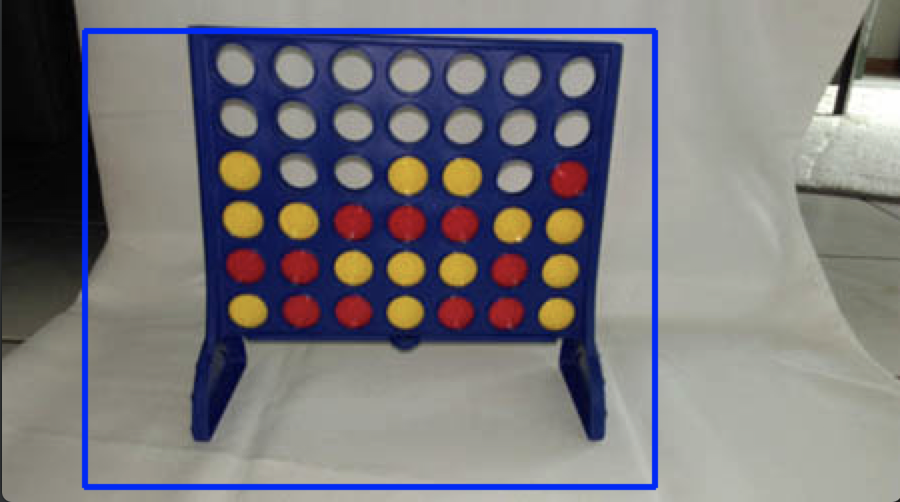
\includegraphics[width = .3\textwidth]{figures/detection.png}
  \caption{Baby in a Magnetoencephalograph. \parencite{babyMEG}}
  \label{fig:meg}
\end{figure}


 by color and pattern comparision.
The image is then cropped and undergoes various image processing steps, such as wrapping, contrast enhancement and color channel extraction.
The current board configuration can then be read and converted to a computer readable format by thresholded color comparision.




%-------------------------------------------------------------------------
\section{Results}

\subsection{Vision}
Processing time is $< 0.3$ s (i7-4790K CPU @ 4.00GHz) per image.


%-------------------------------------------------------------------------
\section{Discussion}

{\small
\printbibliography
}

\end{document}
